\chapter{Search by Object Location}
\label{ch:object_location}

% \todo[inline]{v grafe, na x ovu os dat rank}
% \todo[inline]{\% of searched target images up to a given rank}

\normalem
\emph{You see a picture in your head. Your friend is standing on the beach, and there is a little sandcastle on the left. The sea behind beautifully reflects the sun, which is setting.}
\ULforem

We can imagine that at that particular moment we were shooting a video of the scenery. However, years later, with a vast set of videos in our collections, it may be impossible to re-watch every one of them to find that particular memory. Not all of us can visualize the memory, but about those who can, we say that they have an excellent visual memory \footnote{\url{https://en.wikipedia.org/wiki/Visual_memory}}. We present a technique that can be used to search in a dataset based on such memories of the scenery.

In this chapter, we elaborate approaches for known-item search task based on the visual description of the image. The input is characterized by the way how the objects looked (by providing example images) and their relative location in the image (i.e., top left corner). With that information, we look for a match in the database to the described image. We refer to our input as \emph{collage query}, or simply just as a collage. Collage is created by taking images and placing them onto an empty canvas. The placement of the images also carries a piece of information. We show an example of such a collage (query) in figure \ref{fig:query_collage_comparison}. On the left, we can see a cat in the center behind a window. On the right, we can see a possible visualization of such memory. On the grey canvas, we placed a window, which reminded us of the original one. At the center, we added a similarly colored cat.

\begin{figure}
\centering

\begin{subfigure}[t]{0.45\textwidth}
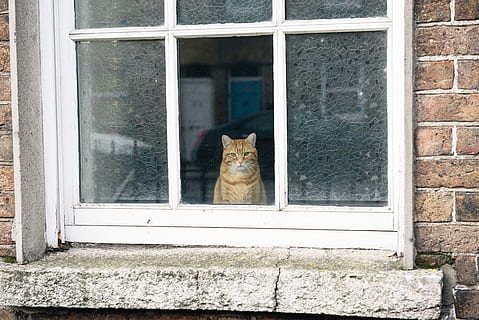
\includegraphics[width=0.9\linewidth]{img/cat_on_window} 
\caption{Target image}
\label{fig:searched_scene}
\end{subfigure}
\begin{subfigure}[t]{0.45\textwidth}
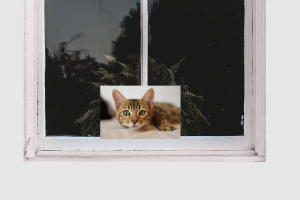
\includegraphics[width=0.9\linewidth]{img/cat_on_window_collage}
\caption{One of the possible collage description of the target image}
\label{fig:collage_example}
\end{subfigure}

\caption{Example of searched image (target) with possible visual description by a collage.}
\label{fig:query_collage_comparison}
\end{figure}

While we were describing the image, we used words for it. However, in this chapter, we do not focus on the search based on the verbal description of the objects. Compared to such a textual approach, we can capture more diversity in the objects by visual information. For example, a single word for a human may represent a visually wide range of possibilities based on clothes, age, and other attributes. On the other hand, these attributes are easier to capture by providing an example image.


This chapter will present three approaches incorporating pre-trained neural networks. We start with the formalization of the task. Next, we provide a short description of user-program interaction and a description of the annotated queries used for evaluations. We use this annotated set of queries to test different sets of hyperparameters and investigate their effect on the system's performance.

\section{Formal description}

In this task we explore the dataset $D$ based on the collage provided by the user. We shall formally define universe of query images as follows: 
$$
    \mathcal{Q} = \{(I, x_0, x_1, y_0, y_1) | I \in \mathcal{U}, x_0 \in [0,1), y_0 \in [0, 1), x_1 \in (x_0, 1], y_1 \in (y_0, 1] \}
$$
where $\mathcal{U}$ is a universe defined in section \ref{s:task_formulation_preliminaries}. $I$ represents an image in the collage; $x_0$, $y_0$ represent the relative position of the top left corner of the image in the canvas; $x_1$, $y_1$ represent the relative position of the bottom right corner of the image in the canvas. Single collage $Q$ is then defined as $Q \subset \mathcal{Q}$

Ultimately, we would like to construct a function $r^*$, that for each query $Q_i \subset \mathcal{Q}$ would find corresponding target image $T_i \in D$. Formally, we can define this function as follows:
$$
    r^*: \mathcal{P(Q)} \rightarrow D 
$$
$$
    r^*(Q_i) = T_i \, \forall (Q_i, T_i) \in X
$$
where $X$ is a set of target images and corresponding queries constructed by the user.

However, due to imperfect user queries, this task maybe even impossible. Therefore, we focus on reordering the dataset, in the way that linear search by the user in this order would provide the target image as quickly as possible. We define \emph{ranking} $r_{D, Q}$ as function with respect to a given dataset $D$:
$$
    r_D: (D \times \mathcal{P(Q)}) \rightarrow \{0, 1, \ldots |D|-1  \}
$$
$$
    \text{ s.t. } \{r_D(d, Q) | d \in D \} = \{0, 1, \ldots |D|-1  \} \, \forall Q \subset \mathcal{Q}
$$

In other words, $r_D(T, Q) = n$ means that target image $T$ is in position $n$ after ordering the dataset $D$ with respect to collage $Q$. This value correlates with the time spend on the linear search of the provided ordered results. This gives us the motivation to evaluate our algorithm based on this \emph{rank} across the whole set $X$.



\section{User-program interaction}

We provide a user with a canvas where they can place, move, and resize the collage images. They can add images by providing an URL of the image, or by pasting the image from a clipboard. One possible way to obtain images for the collage is to use an image search engine (e.g., Google Images). The images can be usually copied to the clipboard by selecting copy in the right-click menu. A quicker approach, we preferred, is using selective screenshots. With the selective screenshot, we can even crop the image, focusing on the part we like, and paste it onto the canvas.

Based on the provided collage, the program searches for similar images in the dataset and interactively presents them back to the user. The user can then alternate the query for a new search, or investigate the displayed results. Figure \ref{fig:query_collage_comparison} shows an example of the query -- the collage of two images (window and cat). 

\subsection{Collected collages}

We manually created a set of queries to evaluate the proposed systems. The annotated data consists of 102 collages, each containing a visual description of a given target image. The average size of the images used in the collages covers 15\% of the canvas. Five percent of the dataset consists of images bigger than 80\% of the canvas. We provide visualizations of the distribution of the annotated queries in figure \ref{fig:annotated_dataset}. Together, all 102 collages are annotated by 199 images.

\begin{figure}
     \centering
     \begin{subfigure}[b]{0.48\textwidth}
         \centering
         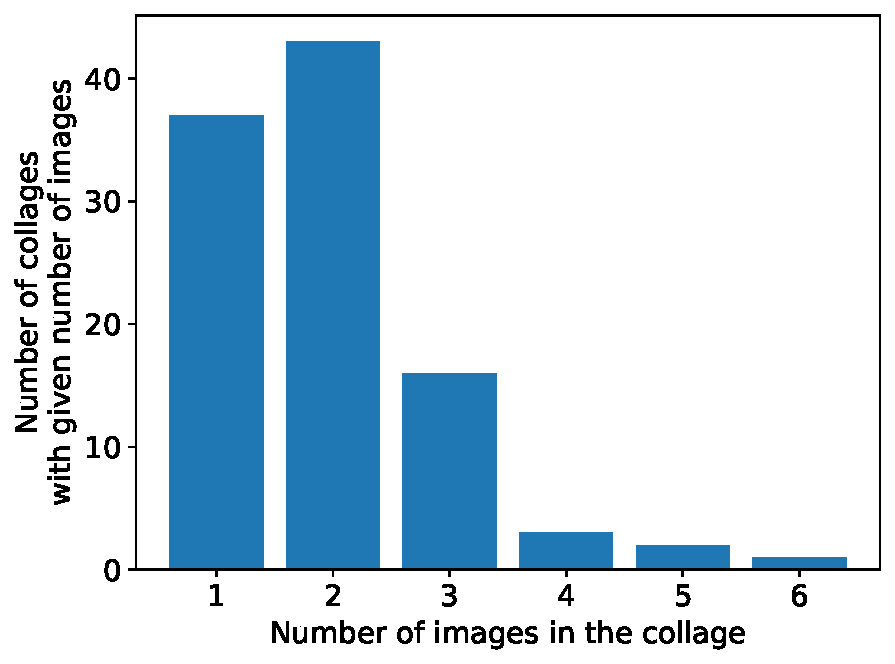
\includegraphics[width=\textwidth]{graphs/num_queries_in_request.pdf}
         \caption{Number of images on a canvas for a collage.}
         \label{fig:y equals x}
     \end{subfigure}
     \hfill
     \begin{subfigure}[b]{0.48\textwidth}
         \centering
         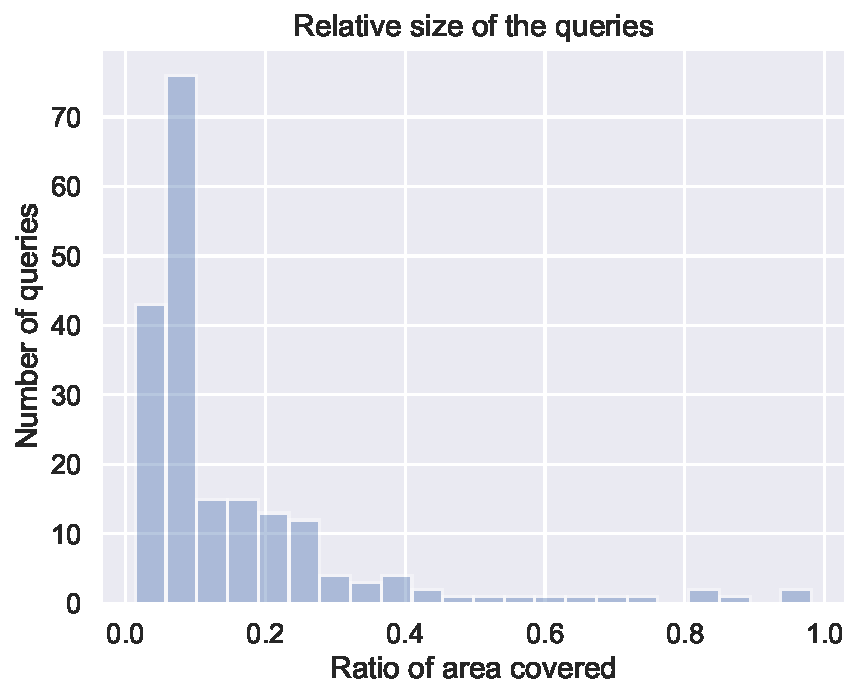
\includegraphics[width=\textwidth]{graphs/queries_size.pdf}
         \caption{Size of the canvas which is covered by a query image.}
         \label{fig:three sin x}
     \end{subfigure}
    
    \caption{Annotated collages properties}
    \label{fig:annotated_dataset}
\end{figure}

For the annotation, we used our application. It is possible to save the collage by clicking ``Submit Collage.'' The average time spent on creating a single collage was 91 seconds. This time includes searching for images online, pasting them onto the canvas, and usually also waiting for the responses of the system.

We want to highlight that we created more than a hundred collages corresponding to the target images from the dataset. The annotations were done only by a one-person. We leave annotation from more people, to study the differences in behavior, for future work. 

\section{Framework overview}

\begin{figure}[p!]
    \centering
    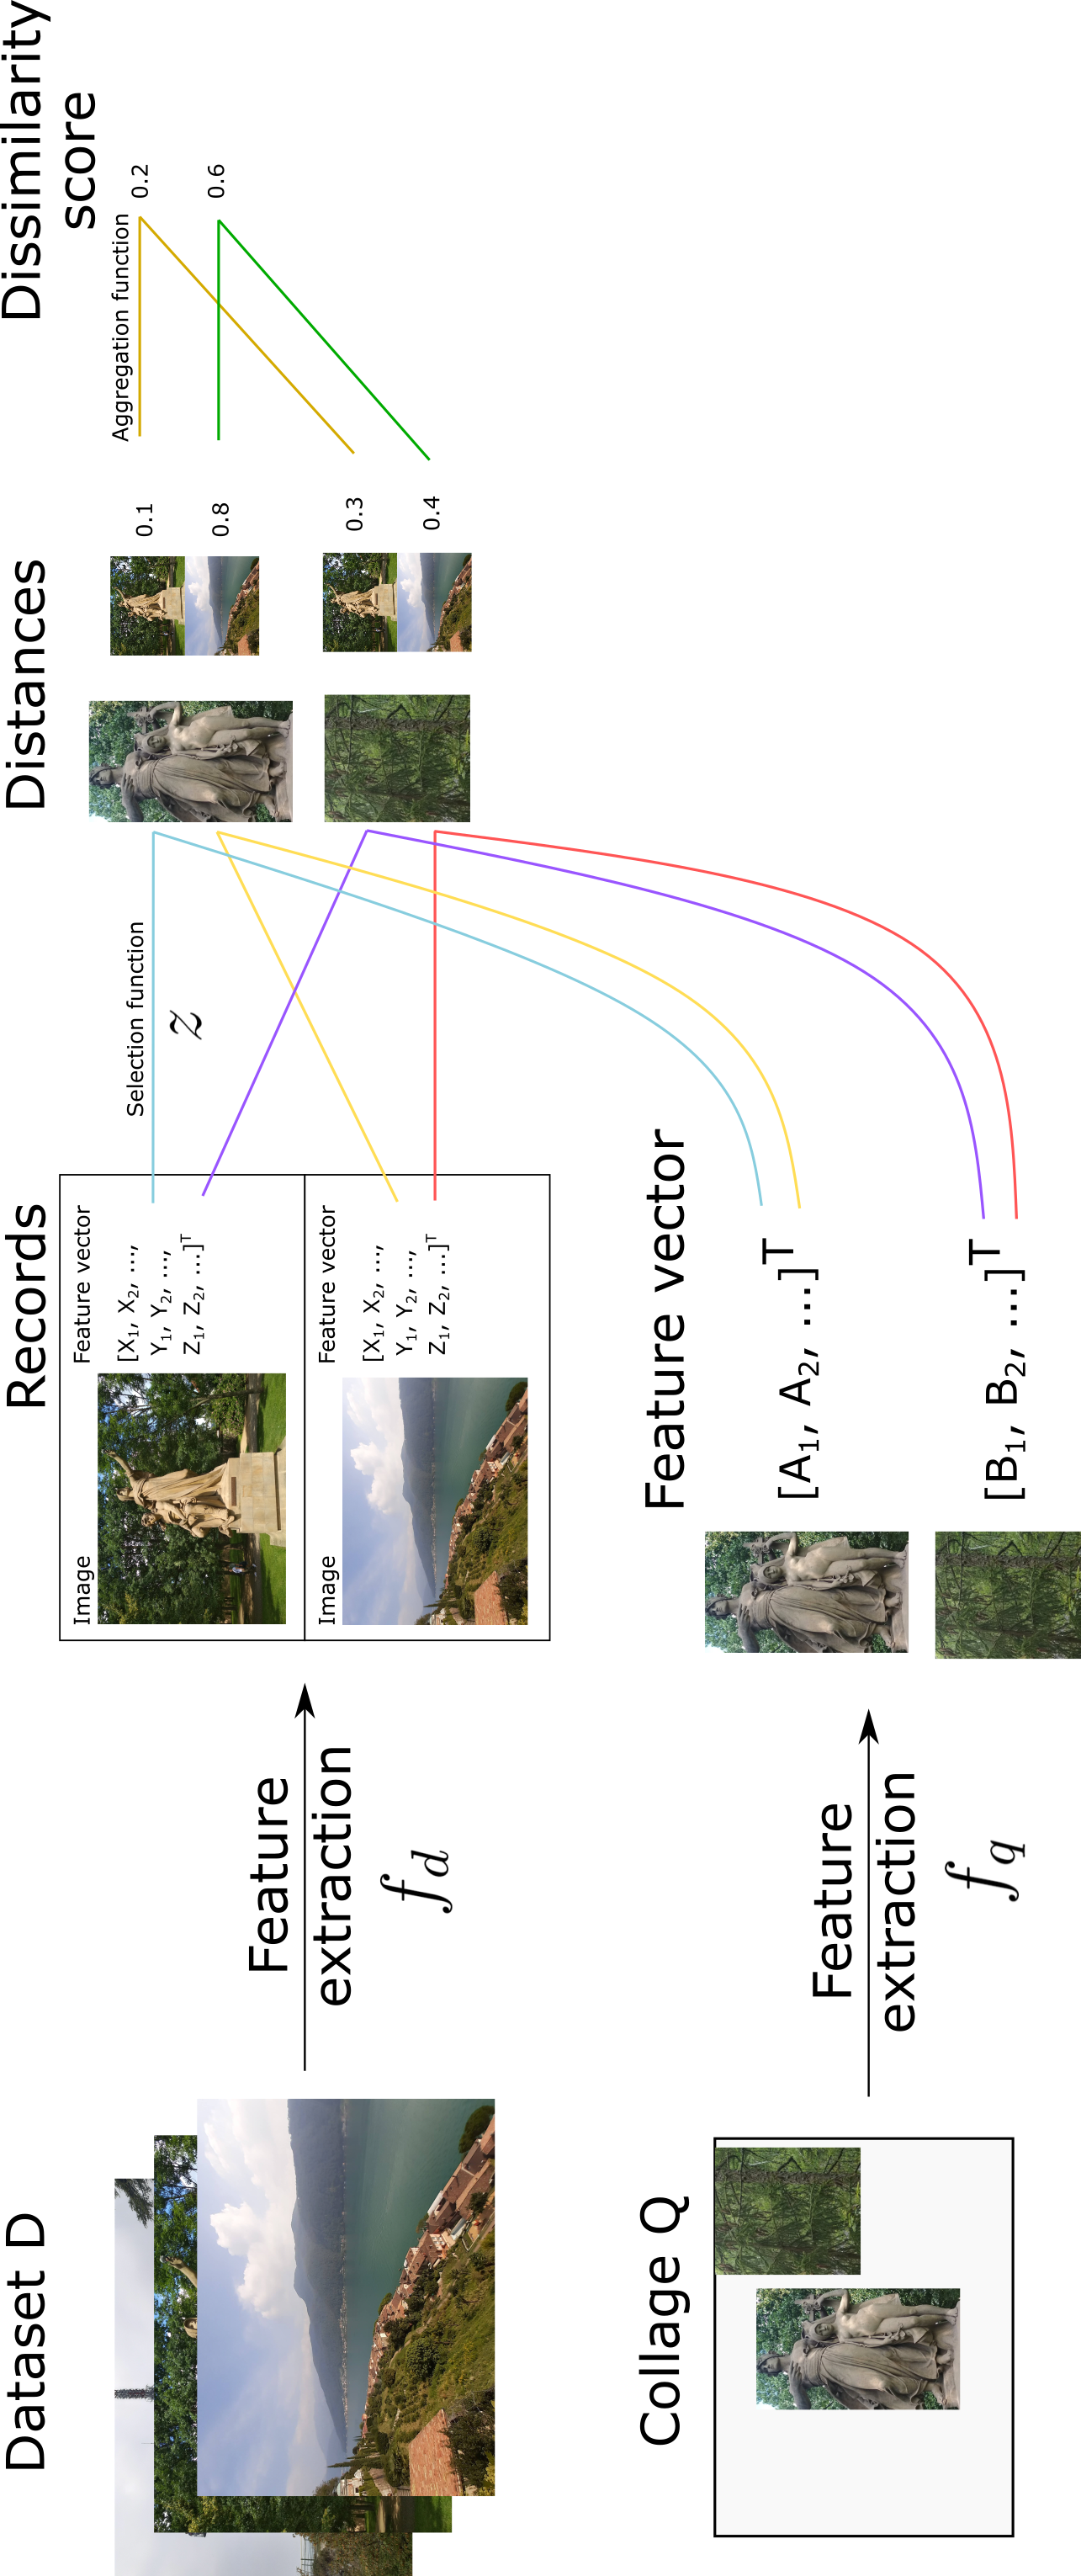
\includegraphics[scale=0.9]{img/features_pipeline.png}
    \caption{Overview of processing pipeline}
    \label{fig:processing_pipeline}
\end{figure}

Our approach consists of several individual steps. Figure \ref{fig:processing_pipeline} shows a visual overview of the steps we describe here. Our first step is to compute feature vectors for each image, given the descriptor. We call this step \emph{feature extraction}. This way, we obtain \emph{records}, i.e., a pair of image from the dataset and its corresponding feature vector. In the figure, we show the possibility of having multiple feature vectors in the same record. Using multiple feature vectors is still following our theoretical model since the space from the concatenation of the feature vectors is isomorph to the $\mathbb{R}^n$. Therefore, we can still think of it as one feature vector. This first step is done only once per descriptor. We obtain the feature vectors offline by a separate module.

In the collage processing path, We use the same descriptor to obtain representations of the images from the query collage. This part is done online; therefore, we have to have the descriptor available for running. Since we only extract features from a couple of images during the run, it is possible to run the prediction by the neural networks on the CPU.

As the next step, our goal is to obtain the distance (dissimilarity) from each query image to each image in the dataset. In our case, we measure the distance between their descriptor representations. Finally, we obtained for each image in the dataset a set of distances to the query collage. Based on these distances, we compute the final \emph{ranking} of the items in the dataset.

While the described pipeline offers a reasonably straightforward approach to the task at hand, the individual stages' internal factors do require a fair amount of tuning. Although we cannot evaluate the performance of the individual steps, we evaluate the hyperparameters with respect to the performance of the whole framework. Throughout the following sections, we progressively build the pipeline while describing the particular approaches we use. We start with the discussion on feature extraction, and then slowly progress towards the next stages of the system.  



% Then, we can measure the queries' success rate, as the number of queries solved up to a given rank. For example, let us have 40 items in the dataset and perform four queries. These queries ranked the target images at the following positions: \{0, 23, 7, 14\}. For a given rank, we are interested in, we compute how many queries were ranked below it. In this scenario, for a rank 20, three queries were ranked lower.

% Since the size of the dataset and the number of tested queries may vary, we always present the results with respect to the size of the set it comes from. In the previous scenario, 75\% of the queries {\color{red} jako ze queries = hledanych objektu? hrozne tezko se to cte a lusti... a to tusim predem, co chcete napsat...} were ranked below the rank representing 50\% of the dataset.

% We use these cumulative, proportional {\color{red} jako ze na ose X se bere \% DB?} results to plot the performance of the framework. A sample evaluation is present in the figure \ref{fig:mobilenet_whole_image_example}. In the case described presented {\color{red} ???????}, 90\% of the annotated collages (queries), the target image was ranked in the first 50\% of the dataset. In other words, this can be said that in 90\% of cases by stating a query, we were able to eliminate half of the dataset as unrelated {\color{red} nechapu co chcete rict...}. We can also notice a steep curve in the beginning. It shows that 70\% of the collages had the target image ranked in the first 10\% of the dataset. We can see that this particular system worked well for 70\% of the collages, but struggled to solve the rest.

% \begin{figure}
%     \centering
%     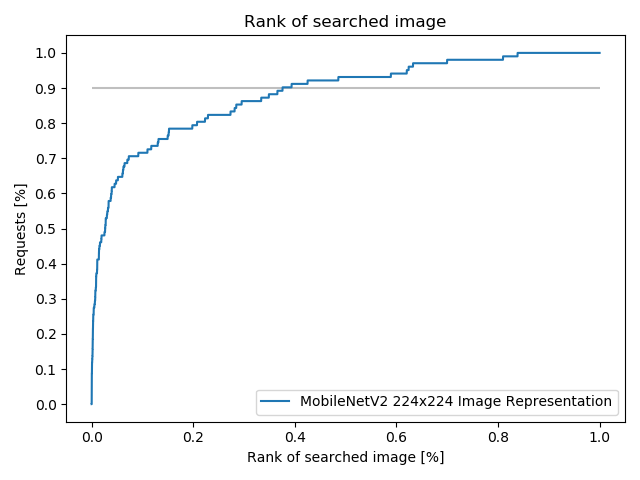
\includegraphics[width=0.8\linewidth]{img/mobilenet_whole_image.png}
%     \caption{Performance of MobileNetV2 on annotated collages}
%     \label{fig:mobilenet_whole_image_example}
% \end{figure}


\section{Features extraction strategies}

In the following section, we present three feature extraction techniques. Recall that the feature extraction technique defines how we extract features for our dataset and our queries. These obtained feature vectors are later used to compute the distance between the provided query image and the dataset image. We kick off this section with the baseline model. In the baseline model, we do not use the spatial information about the images in the collage. This baseline approach is currently used, for example, by the VIRET tool \citep{kovalvcik2020viret}. 

The next two presented approaches elevate the spatial information from the collage. The first one splits the images in the dataset to fixed regions. The second one elevates information from the neural network before the last pooling layer.

\subsection{Baseline -- Image representation}

The baseline ignores the spatial information of the images in the collage. We set this approach as our baseline since it is relatively simple and can solve our task. In this baseline approach, we compute the feature vector for an image in the dataset using a neural network as a descriptor. Since the dimensions of the query images from the collage do not have to correspond to the dimensions of the input of the neural network, we rescale them to the required input size. This method represents an image in the dataset by one feature vector. The collage is then presented by multiple feature vectors, one per query image.

% In figure \ref{fig:mobilenet_whole_image_example}, used for the explanation of the graphs, we show the performance on the annotated set of collages. We present the results on the MobileNetV2. We use MobileNetV2\todo{refy ak nie su niekde vyssie} due to its low computability needs and therefore offering quick annotations {\color{red} spis representation extraction?}. It is widely used in the task, where we expect online or near online evaluation. We included a short description of the Related Work (section \ref{ss:pretrained_models}).

\begin{figure}
\centering
\begin{boxedverbatim}
Dataset:
    - image: 1 feature vector
Query:
    - query_image: 1 feature vector
    - compared to: each feature vector in the dataset
\end{boxedverbatim}
\caption{Overview of the Baseline -- Image representation approach}
\end{figure}

\subsection{Splitting the image into regions}

In the next presented approach, we will focus on using the spatial information of the images in the collage. This position of the objects can serve as highly distinguishing criteria while looking for the target image. In the previous chapter, we described the image in the dataset by only one prediction of the neural network. We obtain higher granularity for the data, by splitting the image into multiple cuts and then obtaining the feature vector on each of the cuts separately.

Assume, we split the image into $m$ cuts. For each image of the dataset, we now need to store $m$ times more information ($m$ feature vectors, one per cut). To avoid increasing the time complexity by the multiplicative factor of $m$, we develop a principle, how to compare the query image only with the one or a few out of these $m$ cuts and not to all. That way, we preserve the same time complexity except for some additive factor, compared to the Baseline.

First we talk about the selection of the cuts, and then we discuss the principle of selection for the cuts. The overview of the information preserved for this approach is in figure \ref{fig:overview_regions}.

\begin{figure}
\centering
\begin{boxedverbatim}
Database:
    - image:
        - multiple crops:
            - crop's position
            - feature vector
Query:
    - query_image: 1 feature vector
    - compared to: only to selected crops from each image
\end{boxedverbatim}
\caption{Overview of the regions' approach}
\label{fig:overview_regions}
\end{figure}

\subsubsection{Cutting the image}

We work with cutting into regions. Each image in the dataset is divided into $N \times M$ regions. Feature representation is then computed and stored for each region separately. The defined cutting is identical for all images in the dataset.

First, we discuss the choice of the shape of the regions into which we want to split the images. Since we plan on feeding the region's image into a CNN, we set a limitation on using only square regions. This limitation comes from the fact that standard CNN architecture expects a square image on the input. We could theoretically rescale rectangular regions into squares, but this would induce a non-necessary distortion of the image. We avoid this distortion by posing this simple condition on the regions' shape.

We test several sizes of the input squares in the experiments. Although, we limit ourselves to the input shapes, for which a pre-trained CNNs are available. This for example for MobileNetV2 includes the following shapes: $96 \times 96, 128 \times 128, 160 \times 160, 192 \times 192$ and $224 \times 224$.

We impose a second limitation on the choice of regions. We require that their union fully covers the input image. In that way, information from each part of the image is extracted in some way. Also, we do not allow the regions to extend over the image. Such an extension would only lead to spending the resources on capturing no ``empty'' information. 

Our limitations summarized are square regions, not extending over the image and full coverage of the input image. Except for a particular case, when the width and height would be divisible by the input shape dimension, there is no cutting, where the regions would not overlap. The special case is not our case since we work with the images $320 \times 180$.

We propose a cutting, which for the desired number of regions $N \times M$ with the desired width $s$ of the region produces evenly distributed regions. We require a non-negative excess $sN - h$, where $h$ represents image height, $s$ the dimension of the CNN, and $N$ number of desired regions over the vertical axis. The excess is evenly split between all regions in the given axis and creates overlaps. Analogously, we handle the horizontal axis.

The side effect of overlaps also plays an important role in this technique. With the rigid frame without overlapping, we could face a situation where a single object would be split into two separate parts. Both parts could lack enough visual information on the object to provide consistent results. With the excess distributed to all regions, we share the information alongside the cut to both regions.

Our fixed parameters are regions' width $s$ and the number of regions we want to use $N \times M$ and image size $h, w$. We solve the task of choosing regions splits for one axis; the second is done analogously. We know that the last region has to end with the edge of the image. Therefore the starting coordinate of the last region is $h - s$. We then split the remaining ``space'' (space not covered by the last region) over $N-1$ regions equally. We call this distance $step$ since it says the distance between the startin points of the regions. The starting coordinate $r_i$ of the $i$-th region in a given axis is:

\begin{align*}
step_h = (h - s) / (N - 1) \\
r_i = {i \, step_h\,\text{for}\,i \in \{0, 1, 2, \dots, N - 1\}}
\end{align*}

With the condition on full coverage of the image (i.e., \(s N >= \text{h}\), and for $M$ respectively), we obtain full coverage of the image by the regions. Overlaps are evenly distributed over both axes. Note that, with bigger sized regions, overlaps may occur between more than two regions. For example, if we split an image with width 180 into three regions with a width of 96 pixels, some areas of the image will be included in all three regions. This happens, when the $step \leq 2 s$.

% We evaluate the performance of the same network using a different number of regions. This experiment is shown in the figure \ref{fig:different_number_regions}. Even though the number of regions was almost doubled (from 8 to 15), we only saw a slight improvement in performance. In the figure \ref{fig:different_region_size} we show the effect of the regions size. We see that the best performing model worked with $2\times4$ regions with the input size of $128\times128$. For this particular setup, it was able to rank 90\% of the collages in the 8\% of the database.

% \begin{figure}
% \centering
% 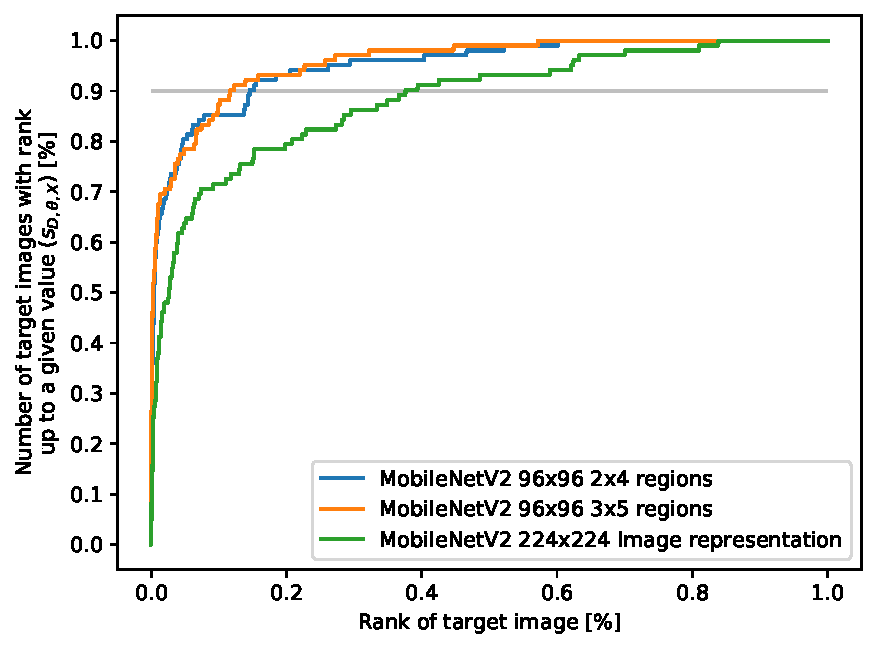
\includegraphics[width=0.8\linewidth]{graphs/0c36458e4a7754f349e4dd02e823acc5f192f0aaa42647313045530525f3db19.pdf}
% \caption{An experiment comparing the effect of the changing number of regions.}
% \label{fig:different_number_regions}
% \end{figure}

% \begin{figure}
% \centering
% 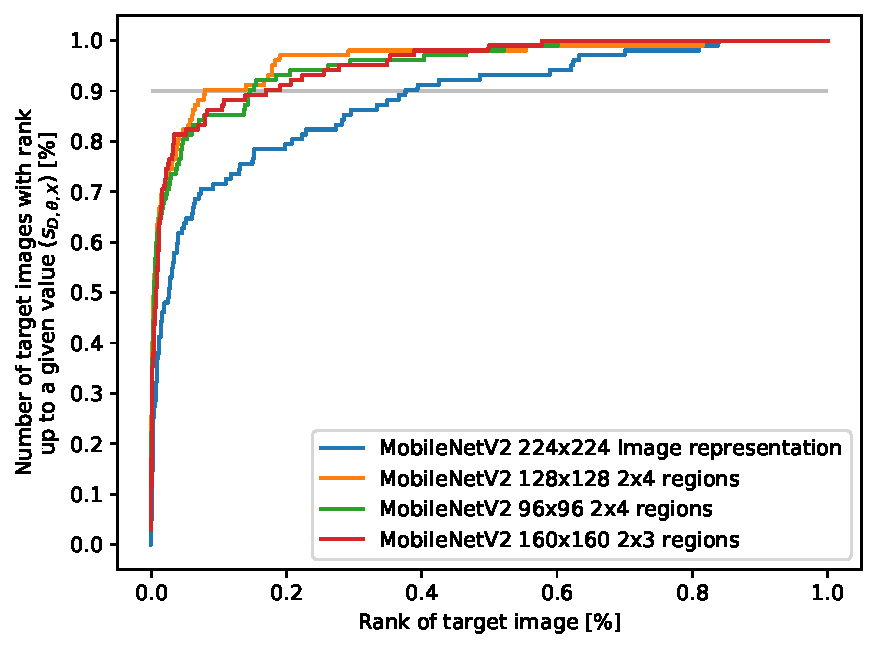
\includegraphics[width=0.8\linewidth]{graphs/901175c0015f71987720d10953133afa566d88a09a6d7182a074859ff4e8409e.pdf}
% \caption{An experiment comparing the effect of the changing regions size.}
% \label{fig:different_region_size}
% \end{figure}


\subsubsection{Selecting regions}

Previously, we defined cutting into the regions for each item in the dataset. One of the possible steps further in the pipeline could be to compare all regions' feature vector to the query image feature vector. Although this would be an entirely valid approach, it has two caveats: firstly, it does not take advantage of knowing the position of the query image in the collage, and secondly, it multiplicatively increases the time required, when comparing to $N \times M$ more feature vectors, than before.

We discuss the options of selecting only relevant regions to the query image based on the position of the query image. Given one incoming query image with its position and shape, we propose the following methods for choosing the relevant regions:
\begin{itemize}
  \item choosing only the one, which is covered the most,
  \item choosing all regions, which have a non-empty intersection with the query
  \item or approaches in between, by setting a maximum to a number of relevant regions.
\end{itemize}

We visualize the problem in the figure \ref{fig:fish_with_grid}. The query would be an image of the fish placed as the red boundary shows. All regions with a nonempty intersection with the query image are highlighted in green. The region with the highest ``coverage'' is the blue one.

To make this idea over coverage measurable, we use the Jaccard index. We compute the Intersection over Union between the region and the crop, where is the query image located. 

\emph{Intersection over Union} (also known as Jaccard index\footnote{\href{https://en.wikipedia.org/wiki/Jaccard_index}{https://en.wikipedia.org/wiki/Jaccard\_index}}) measures similarity between two sets. We use it as a metric to express how much two regions (i.e., two rectangles) overlap. 

The definition of the Intersection over Union is following:
$$
    J(A, B) = 
    \begin{cases}
      1, & \text{if\ A and B are empty} \\
      \frac{|A \cap B|}{|A \cup B|}, & \text{otherwise}
    \end{cases}
$$

In our case, the $|A \cap B|$ represents the area that belongs to both region and query image. The  $|A \cup B|$ represents the area covered by the union of both. A visual representation of the formula is displayed in the figure \ref{fig:intersection_over_union}. Using this index, we can order the regions based on their coverage with the query image. The more relevant are the ones with the higher Intersection Over Union and vice versa.

\begin{figure}
    \centering
	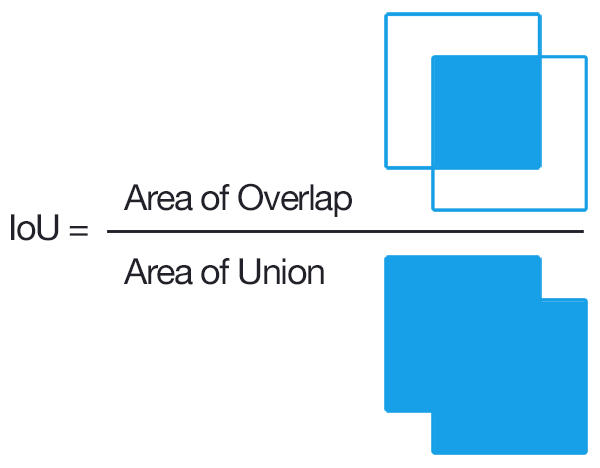
\includegraphics[width=0.3\linewidth]{img/Intersection_over_Union_-_visual_equation.png}
	\caption{Intersection over Union between regions. Source: Wikipedia, CC BY-SA 4.0}
	\label{fig:intersection_over_union}
\end{figure}

With the selected regions, we compute the distance between the query image and each of the regions. For each record from the dataset, we select only one region with the lowest distance to the query.

From the regions ordered by their IoU to the query image, we select the first $n$, based on the strategy. Recall that the required output of this stage is only one distance and not multiple from multiple regions. Therefore, when we compare the feature vectors with multiple regions, we select only a winner with the lowest distance for the next phase. 

% We present an experiment, where we took all intercepted regions (green regions in the example), only the region with the highest IoU (blue region in the example), or equivalently first 2 with the highest IoU or first three regions. The results of the experiment are shown in figure \ref{fig:crop_limitation}. In the results, we see no significant improvement in any of the provided choices. Although, the selection of only the region with the highest overlap gives us the least computable heavy\todo{mozno nieco ine ako heavy - bud hard ak to fakt je np-tazke alebo nieco typu demanding} approach.

\begin{figure}
\centering
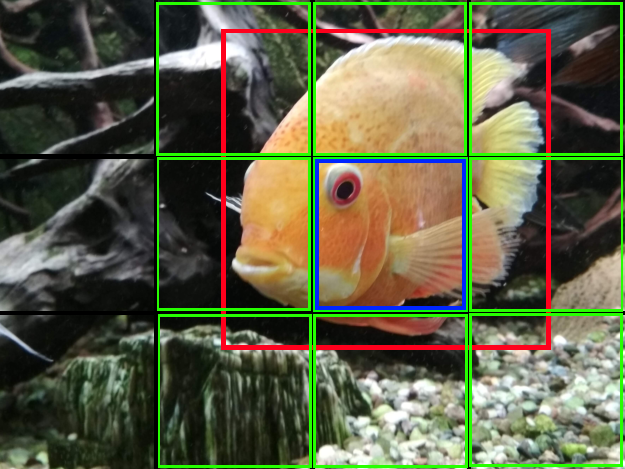
\includegraphics[width=0.6\textwidth]{img/fish_grid_regions}
\caption{Example of choosing the corresponding regions. Red: query position; Green: all intercepted regions; Blue: region with highest IoU.}
\label{fig:fish_with_grid}
\end{figure}


% \begin{figure}
% \centering
% 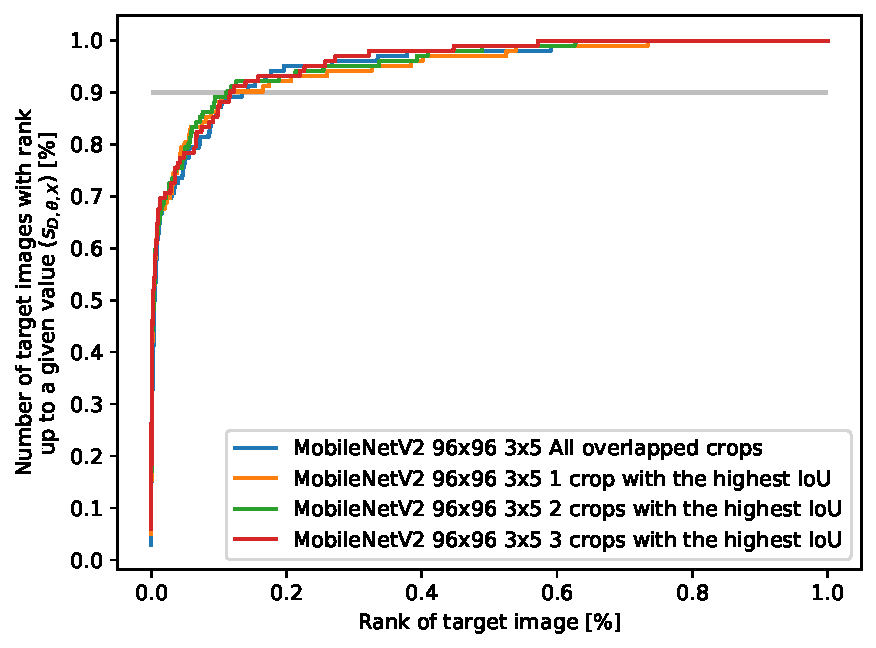
\includegraphics[width=0.8\linewidth]{graphs/5c4a781f8e6f3eac93db2083bde3963c06582a92a8141411bf29e41251a98e75.pdf}
% \caption{Performance of the system based on different number of chosen crops}
% \label{fig:crop_limitation}
% \end{figure}

\subsection{Using the representation before pooling}

The disadvantage of the previously presented technique is fixed cutting. The cutting into regions does not adapt to the size of the input query. 

Let us retake a look at the fish in figure \ref{fig:fish_with_grid}. We can see that fish covers approximately two-thirds of the image, but the individual regions cover only one-twelfth. In this case, only this one-twelfth of the image is compared to the query image. The method is missing any adaptation on the size of the query image.

After investigating the structure of the CNNs, we propose an approach based on the information obtained in the last convolution block. In standard architectures, after the last convolution block follows the pooling layer. So far, we worked only with the representation based on this pooling layer. Since we have stripped two layers from the classification CNN -- the fully connected layer used for classification, and the pooling layer, we also refer to this method as ``antepenultimate'' -- last, but two.

Since the results we now work with are obtained before global pooling, i.e., from the last convolution block, they have a different shape. The space of the featurre vectors is now $\mathbb{R}^{k\times l \times c}$. Typically, this space is reduced to $\mathbb{R}^c$ by the global pooling layer.

Due to the way how CNNs work, we assume we could use the information about the query position, to work only with the part of the results provided by the antepenultimate layer. The overview of the method is available in figure \ref{fig:antepenultimate_overview}

\begin{figure}
\centering
\begin{boxedverbatim}
Database:
    - image:
        - 1 feature vector (the result before pooling):
Query:
    - query_images: global average pooling over feature vectors
    - compared to: pooling over selected region
\end{boxedverbatim}
\caption{Overview of the using the representation before pooling}
\label{fig:antepenultimate_overview}
\end{figure}


\subsubsection{Choosing a region of interest in the layer}

Layer before pooling on which we focus (antepenultimate) is the last convolution block. Therefore, it produces features from space $\mathbb{R}^{n\times m \times c}$, where $n, m, c$ is the shape of the convolution block. The first two dimensions contain spatial information, which is propagated from the previous layers. The third represents the channels (i.e., features).

To obtain only a part of this layer, we are interested in (i.e., our query was placed in that specific region); we need to take only a subset over the first two dimensions. For a query defined by region $R_i = (y, x, h, w)$ and a hidden layer $L_i$ with dimensions $(H, W, C)$ we consider select following subset of the layer: $L_i[y * H: (y+h) * H][x*W, (x + w) * W][:]$. We use a notation that, for a given dimension, $:$ represents a half-open interval. If there are no limits, then it represents taking the vector fully in a given dimension.

Both MobileNetV2 and Resnet50V2 end with a convolution block with dimensions $(7,7,C)$, where $C = 1280$ for MobileNetV2 and $C = 2048$ for Resnet50V2. Previously mentioned selection of interesting regions may result in empty selection. For example, when the query image covers only one-tenth of the image in both dimensions. The rounding may result in an empty interval. We solve by adding one to the dimension, whenever it would be empty.

Now, we selected a subset of the last convolutional block. The original network follows with \verb+GlobalAveragePooling2D+. We perform the same operation on the selected subset. This way, we again obtain the feature vector from $\mathbb{R}^c$ for each record.

Compared to the previous approaches, we aim to avoid strict cutting and provide more flexibility. On the other hand, this approach requires more memory since we store 49 feature vectors per vector ($7\times7$). We present the results in figure \ref{fig:antepenultimate}. Due to its memory limitation, we downsized the dataset to one-tenth. We randomly sampled the images from the dataset. We provide a baseline on this smaller dataset. We can see an improvement compared to the baseline. We were able to implement spatial information of the query successfully. However, the performance is worse compared to one of our region's techniques. We assume that this is caused by the fact that running a network 15 times can extract more information than running it only once.

\begin{figure}
    \centering
    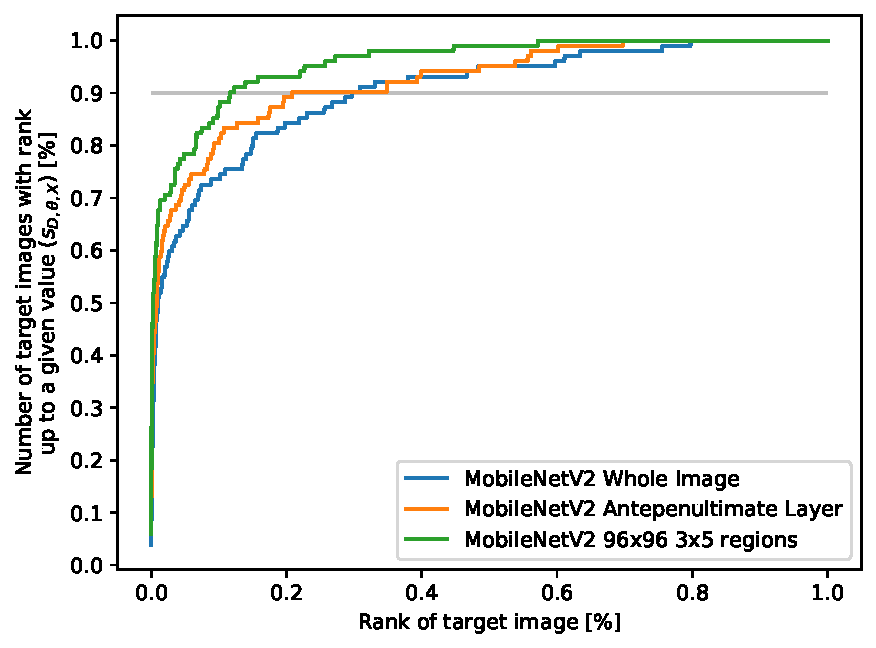
\includegraphics[width=0.8\linewidth]{graphs/adaf8d435bb40406f9ce40654ec396e04453ab76cf0776d2a87d385055d5424f.pdf}
    \caption{Comparison of baseline, regions and aproach using the antepenultimate layer.}
    \label{fig:antepenultimate}
\end{figure}

\section{Ranking}

Let us remind an overview from figure \ref{fig:processing_pipeline}. In the previous sections, we have seen two approaches presented for feature extraction. The first one was based on the regions, the second one based on the antepenultimate layer from CNN. Now we will\todo{bez buduceho casu} continue in the second part of the pipeline, extracting distances and ranking the records in the database. We continue to work with our so far best-performing model -- MobileNetV2 spitted into 2x4 regions with the input size 128x128.

In the previous sections, we talked about obtaining feature vectors for the items in the database while selecting only relevant regions. In this section, we take a closer look at further processing these obtained feature vectors.

We extract features for query images the same way (using the same model) for the items in the dataset. Then, we compute the distance between the query image and the items in the dataset for each query image.

Based on these distances, we order the results, starting from the smallest distance. This distance acts as an inverse for the similarity. More similar the results are, the smaller is the distance.

In figure \ref{fig:regions_distances}, we show a comparison between three different distance measures we compared. We see a superior performance of the cosine distance over Euclidean and Manhattan distance. Since we work with a high dimensional space (in case of MobileNetV2, it produces 1280 dimensions after pooling), the Euclidean distance suffers from the curse of the dimensionality\footnote{\url{https://en.wikipedia.org/wiki/Curse\_of\_dimensionality\#Distance\_functions}}. 

\begin{figure}
    \centering
    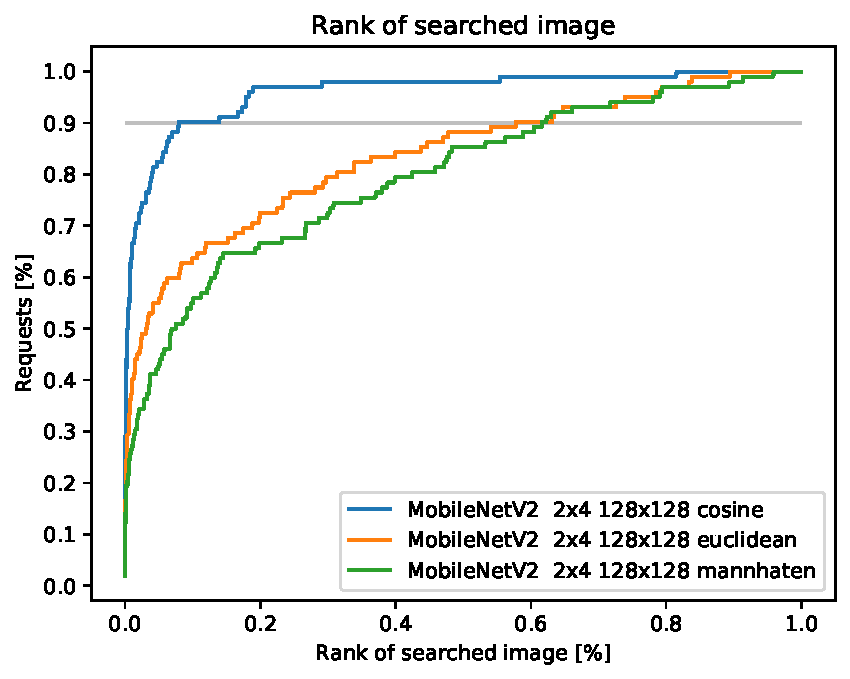
\includegraphics[width=0.8\linewidth]{graphs/3aab502ea602a9f49afaa0a0d998cf226a0a67b9efcaa655d2ddf5063eeabe47.pdf}
    \caption{Comparison of the performance based on the chosen distance function.}
    \label{fig:regions_distances}
\end{figure}

\section{Multiple objects in the scene}

We already discussed techniques for feature extraction and distance. We produced the ranking of the dataset for each query image. In this section, we solve a question of how to merge these rankings from multiple query images to obtain one final ranking, which is presented to the user.

For our task, we do not assign any weights to the input query images. We neither work with the order of their placement. A collage is an unordered set of images with their location. In this section, we assume we already have the ranks per query image. Our goal is to merge them and produce one ranking.

We define ranking $R$ as a set of distances between the query image $q$ and database item $i$. We look for a function $r: R^n \rightarrow R$, which merges multiple rankings into one final ranking.

We test three such functions, $min(\cdot)$, $mean(\cdot)$ and $max(\cdot)$.  For a database image, we compute the distance as a given function from the distances to the query images. Afterward, we rank the database images based on their distances. 

A comparison of these functions for MobileNetV2 can be seen in figure \ref{fig:ranking_funcs}. The $min(\cdot)$ has the advantage of "forgiving" if some of the images provided in the collage were unrelated. The $max(\cdot)$, on the other hand, ranks the images based on the worst match. As our results show, it best performs $mean(\cdot)$, as it assigns the importance to each image from the collage equally.

\begin{figure}
\centering
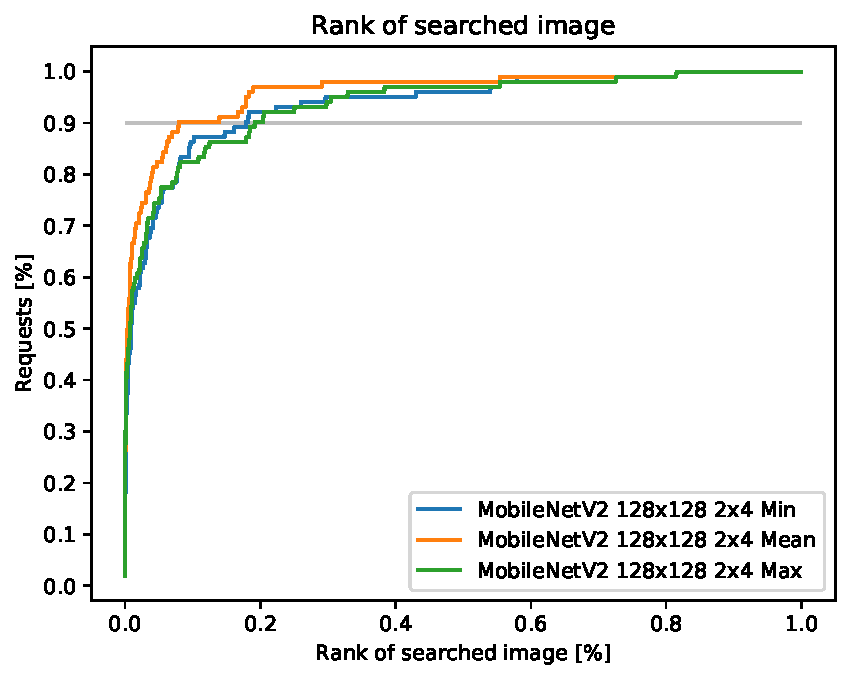
\includegraphics[width=0.8\linewidth]{graphs/70c56dc52be92e048f57b9bdfb35ddce2be41fd2454ae360588da2e387b09de5.pdf}
\caption{Performance of the system based on different ranking function}
\label{fig:ranking_funcs}
\end{figure}

\section{Padding}

We talked about the importance of the square input in the Regions section. During the development, we also explored preprocessing techniques for query images.

Our input to the network is a square. From the user's point of view, we support rectangles. The option to create non-square queries comes handy when the user wants to include, for example, a picture of a person standing, or kayak. A question arises, what is the best way to edit the image to fulfill the square requirement. We test three techniques: rescale, black padding, and white padding. The disadvantage of the rescale is that it distorts the proportions. If the person in the query image is in a tall and narrow box, the distortion will cause it to appear more full and shorter. The distortion becomes stronger with an increasing imbalance between the box dimensions. 

Our question \todo{duplicita - The following experiment compares the approaches of ...} is if it is better to distort the image or provide the image with padding to fill the square shape. For almost square images, the padding covers only a small portion of the image. For images with a significant imbalance in the dimensions, it includes much space with no useful information for the network. A second question we ask is if the color of the padding results in different performance.

The results are shown in figure \ref{fig:padding}. We can see that a rescaling achieved the best performance. A small improvement is achieved by using white padding instead of black. Since the results show favor in rescale, we use it for all other experiments.

\begin{figure}
    \centering
    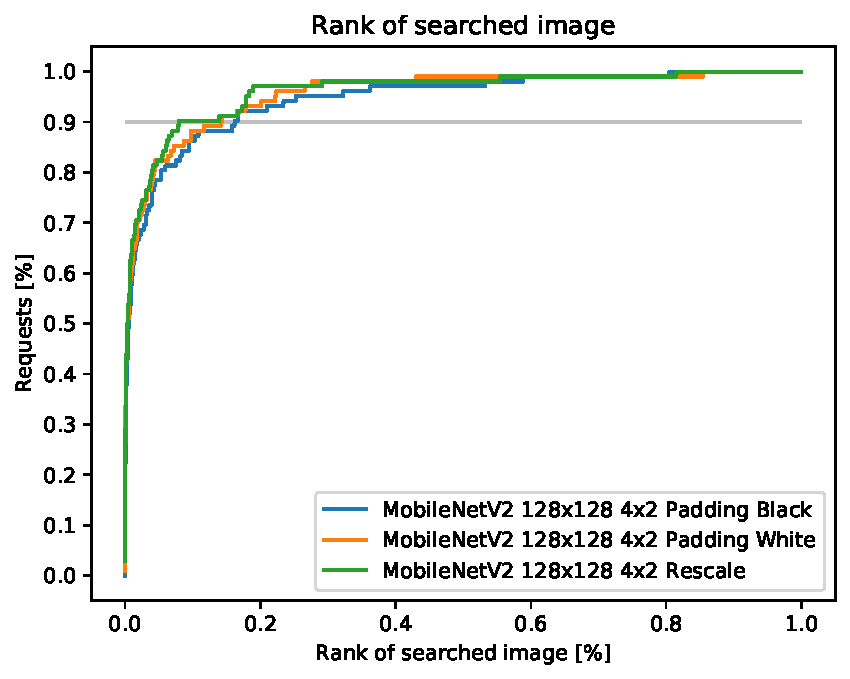
\includegraphics[width=0.8\linewidth]{graphs/bf57efafbbbc7b5a1744054d87d4ecfa381c9eaf2459186904190d97bcb99a81.pdf}
    \caption{Comparison of different padding method for images in the query.}
    \label{fig:padding}
\end{figure}

\section{Dimensionality reduction}

In the previous sections, we evaluated several hyperparameters of the system to achieve the best performance. In this section, we take a look at reducing the dimensionality of the extracted features. Dimensionality reduction could help us to scale our approaches to even bigger datasets and to decrease the query response time.

The extracted features from the neural networks are from high-dimensional space (for MobileNetV2, it is 1280 features, for Resnet50 it is 2048 features). \todo{Moreover, ...}The dimensionality reduction can also have a positive effect on reducing noise if present in the feature vector. We test the performance of the system based on the number of features used. We use the Principal Component Analysis \todo{ref?} for dimensionality reduction. The results are shown in figure \ref{fig:pca}. From the results, we can have several interesting observations.\todo{The results offer several...} Even with as low as eight components (8 features), we can obtain performance \todo{comparable to the} as the original Image representation baseline. With the increasing number of components, the system performs better. With 512 components, it even performed slightly better as the original data. For our purposes, we think \todo{conclude / nieco viac scientific ako think} that selecting 128 components offer the best performance-cost ratio. With the need for smaller feature vectors, we would select at minimum 64.

\begin{figure}
    \centering
    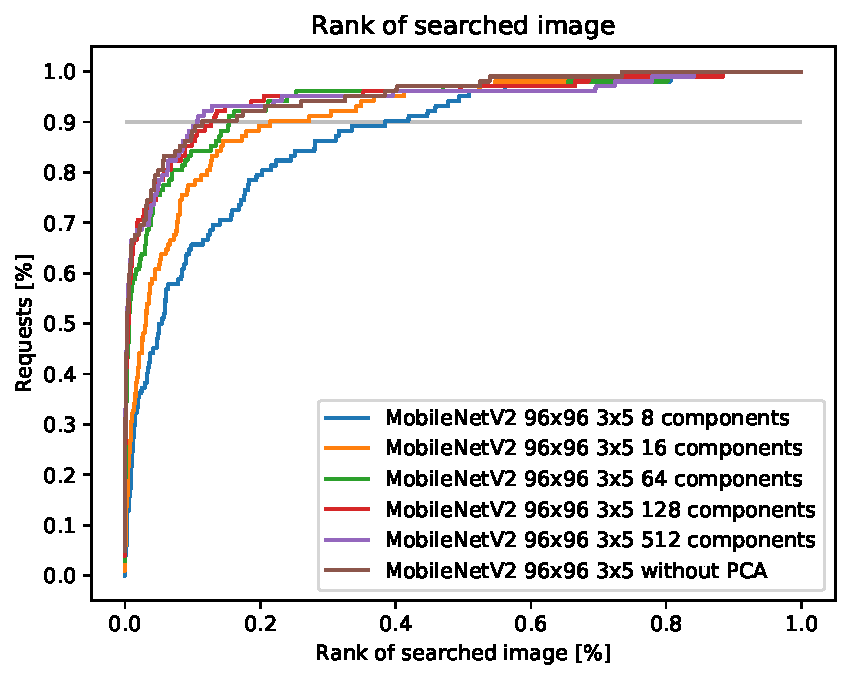
\includegraphics[width=0.8\linewidth]{graphs/6fbd4f70810e1f63f400ef601c1cdba0fd1635749810aa2347a4ff26e6fccf47.pdf}
    \caption{Effect of PCA on the performance of the system}
    \label{fig:pca}
\end{figure}

\section{Neural network selection}

In the previous experiments, we always used MobileNetV2 as our feature extraction model. Thanks to that, we were able to retrieve the best set of hyperparameters for this KIS task. As our last experiment in this chapter, we evaluate the effect of the model on the framework's performance.

In figure \ref{fig:networks}, we present a comparison between the three models. We used two different instances of the ResNet, Resnet50, and Resnet50V2. Networks widely available pre-trained are usually trained on the ImageNet challenge. The task in the challenge is to classify into 1000 classes. In this manner was trained MobileNetV2 as well as Resnet50V2 we used \todo{The ... were trained in this manner alebo proste iny slovosled}. We present the Resnet50 as model pre-trained on more than eleven thousand classes. We aim to support the claim experimentally that network trained on more classes can achieve a better performance level. \todo{paragraf?} In the experiment, we can see that both ResNets work better than MobileNetV2. At the same time, we can see that ResNet trained on more classes performed significantly better in the beginning. Although, we have to note that Resnet50V2 was more successfully solving the rest of the queries.

The downside of using a ResNet50 trained on eleven thousands of classes compared to MobileNetV2 is slower evaluation and availability. Since this is not the challenge,\todo{bez tejto ciarky} the researchers focus on most, the set of pre-trained neural network for this task is smaller. Also, \todo{the} used Resnet50 is only pre-trained with the input shape 224x224. To use it for the regions, we introduced upscaling for the network input. Even though \todo{even with, alebo nieco ine} these difficulties, it proved itself as the best choice out of the compared alternatives.

\begin{figure}
    \centering
    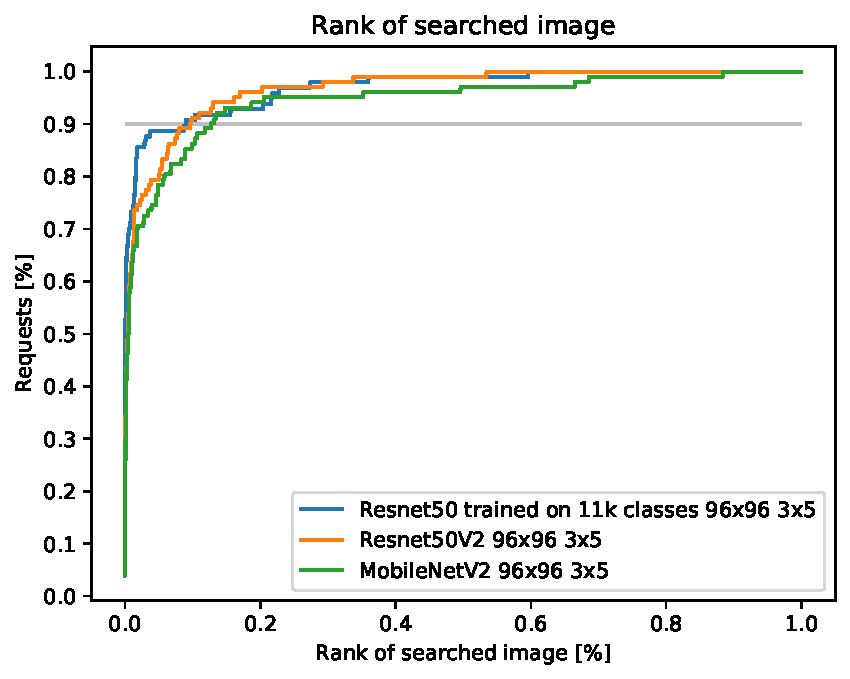
\includegraphics[width=0.8\linewidth]{graphs/2536f6c96149dea24dae84dbf52f760d7d58b0dffa7d660656e1784d9dca277f.pdf}
    \caption{Comparison of the performance based on different feature extraction models.}
    \label{fig:networks}
\end{figure}

\section{Overview of the achieved results}

In this chapter, we tested several hyperparameters for this task. We experimentally proved their validity. The best performing approach was cutting into regions. The setting of \emph{2x4 regions 128x128}, as well \emph{3x5 regions 96x96} performed both well. We found out that the number of selected crops does not have a significant role in improving the searched image's rank. For the distance function, we chose \emph{cosine distance} since it performed significantly better than the others. To merge the rankings, we continue with the \emph{average}. For the padding selection, it emerged from the experiment that \emph{rescale} worked the best. The next hyperparameter, we obtained, is that dimensionality reduction into \emph{128} (ten times smaller than original ones) has almost no effect on the system's performance. From the tested networks, \emph{Resnet50} trained on eleven thousands of classes performed the best.

\todo{In this chapter, we focused on fine-tuning several hyperparameters of the task at hand. We achieved the best results using the approach of cutting the image into regions, with settings of 2x4 and 3x5 regions both achieving good results. Additionally, we...}

\todo{Finally, we concluded that dimensionality reduction into...}